\documentclass[../../../main.tex]{subfiles}

\begin{document}
\begin{multicols}{2}[\section{Fundamentals of mathematics}]
    \subsection{Introduction}
    \textcolor{green}{FALTA COSA}
    \subsection{Set theory}
    \begin{definition}
        A \textit{set} is a collection of distinct elements.
    \end{definition}
    \begin{definition}
        Let $A$ be a finite set. The \textit{cardinal of $A$}, $|A|$, is the number of elements in $A$.
    \end{definition}
    \begin{definition}
        Let $A$ be a set. We say a set $B$ is a \textit{subset} of $A$, denoted by $B\subseteq A$, if and only if all elements of $B$ are also elements of $A$
    \end{definition}
    \begin{definition}[Axiom of extensionality]
        Let $A$, $B$ be two sets. We say that $A$ and $B$ are \textit{equal}, $A=B$, if and only if $A\subseteq B$ and $B\subseteq A$.
    \end{definition}
    \begin{definition}
        Let $A$ be set. The subset $\mathcal{P}(A)$, called \textit{power set}, is the set of all subsets of $A$.
    \end{definition}
    \begin{definition}
        We define the \textit{empty set} $\emptyset$ as the unique set having no elements.
    \end{definition}
    \begin{definition}
        Let $A$, $B$ be two sets. The \textit{intersection of $A$ and $B$}, $A\cap B$, is the set of all elements of both $A$ and $B$. That is, $$A\cap B=\{x:x\in A\text{ and }x\in B\}.$$
    \end{definition}
    \begin{prop}
        Let $A$, $B$, $C$ be three sets. Then:
        \begin{enumerate}
            \item $A\cap B=B\cap A$.
            \item $A\cap(B\cap C)=(A\cap B)\cap C$.
            \item $A\cap B\subseteq A$.
            \item $A\cap\emptyset=\emptyset$.
            \item $A\subseteq B\iff A\cap B=B$.
            \item If $C\subseteq A$ and $C\subseteq B$, then $C\subseteq A\cap B$.
        \end{enumerate}
    \end{prop}
    \begin{definition}
        Let $A$, $B$ be two sets. The \textit{union of $A$ and $B$}, $A\cup B$, is the set of all elements of either $A$ or $B$. That is, $$A\cup B=\{x:x\in A\text{ or }x\in B\}.$$
    \end{definition}
    \begin{prop}
        Let $A$, $B$, $C$ be three sets. Then:
        \begin{enumerate}
            \item $A\cup B=B\cup A$.
            \item $A\cup(B\cup C)=(A\cup B)\cup C$.
            \item $A\subseteq A\cup B$.
            \item $A\cup\emptyset=A$.
            \item $A\subseteq B\iff A\cup B=B$.
            \item If $A\subseteq C$ and $B\subseteq C$, then $A\cup B\subseteq C$.
        \end{enumerate}
    \end{prop}
    \begin{prop}
        Let $A$, $B$, $C$ be three sets. Then:
        \begin{enumerate}
            \item $A\cap (B\cup C)=(A\cap B)\cup (A\cap C)$.
            \item $A\cup (B\cap C)=(A\cup B)\cap (A\cup C)$.
        \end{enumerate}
    \end{prop}
    \begin{definition}
        Let $U$ be a set and $A\subseteq U$ be a subset of $U$. The \textit{complement of $A$ in $U$} is the set of elements not in $A$. That is, $$A^c=\{x\in U:x\notin A\}.$$
    \end{definition}
    \begin{prop}[De Morgan's laws]
        Let $U$ be a set and $A$, $B$ be two subsets of $U$. Then:
        \begin{enumerate}
            \item $(A\cup B)^c=A^c\cap B^c$.
            \item $(A\cap B)^c=A^c\cup B^c$.
        \end{enumerate}
    \end{prop}
    \begin{definition}
        Let $U$ be a set and $A$, $B$ be two subsets of $U$. The \textit{set difference of $A$ and $B$}, $A\setminus B$, is the set of elements in $A$ but not in $B$. That is, $$A\setminus B=\{x\in A:x\notin B\}.$$
    \end{definition}
    \begin{prop}
        Let $A$, $B$, $C$ be three sets. Then:
        \begin{enumerate}
            \item $A\setminus B=A\cap B^c$.
            \item $C\setminus(A\cap B)=(C\setminus A)\cup (C\setminus B)$.
            \item $C\setminus(A\cup B)=(C\setminus A)\cap (C\setminus B)$.
        \end{enumerate}
    \end{prop}
    \begin{center}
        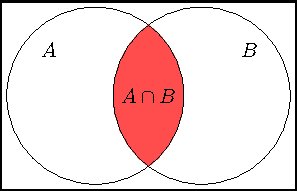
\includegraphics[width=0.49\linewidth]{Images/intersection.tex}\hfill
        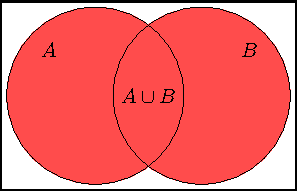
\includegraphics[width=0.49\linewidth]{Images/union.tex}\\
        \vspace{0.02\linewidth}
        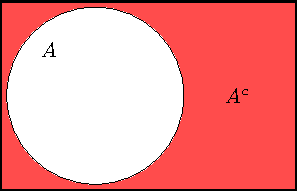
\includegraphics[width=0.49\linewidth]{Images/complement.tex}\hfill
        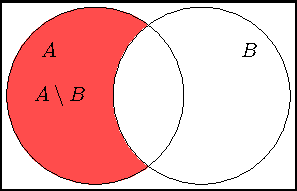
\includegraphics[width=0.49\linewidth]{Images/difference.tex}
        \captionof{figure}{Venn diagrams}
    \end{center}
    \begin{definition}
        Let $A$, $B$ be two sets. The \textit{Cartesian product}, $A\times B$, is the set $$A\times B=\{(a,b): a\in A\text{ and }b\in B\}.$$
    \end{definition}
    \begin{prop}
        Let $A$, $B$, $C$ be three sets. Then:
        \begin{enumerate}
            \item $A\times \emptyset=\emptyset\times A=\emptyset$.
            \item $A\times(B\cap C)=(A\times B)\cap(A\times C)$.
            \item $A\times(B\cup C)=(A\times B)\cup(A\times C)$.
        \end{enumerate}
    \end{prop}
    \begin{definition}
        Let $A$, $B$ be two sets. A \textit{function from $A$ to $B$} is a binary relation between $A$ and $B$ that associates to each element of $A$ exactly one element of $B$.
    \end{definition}
    \begin{definition}
        Let $A$, $B$, $C$ be three sets and $f:A\rightarrow B$, $g:B\rightarrow C$ be two functions. The \textit{composition $g\circ f$} is:
        $$\begin{array}{r@{\hspace{0.5\tabcolsep}}c@{\hspace{0.5\tabcolsep}}c@{\hspace{0.5\tabcolsep}}c@{\hspace{0.5\tabcolsep}}c}
            g\circ f:A&\longrightarrow & B & \longrightarrow &C\\
            a&\longmapsto & f(a) & \longmapsto & g[f(a)]
        \end{array}$$
    \end{definition}
    \begin{definition}
        Let $f:A\rightarrow B$ be a function and $U\subseteq A$ be a subset. The \textit{image of $U$} is the subset of $B$ defined by $f(U)=\{f(u): u\in U\}$. If $U=A$, $f(U)=f(A)=:\im f$ is the \textit{image of $f$}.
    \end{definition}
    \begin{definition}
        Let $f:A\rightarrow B$ be a function and $b\in B$. The \textit{preimage of $b$} is the set of elements $a\in A$ such that $f(a)=b$. More generally, if $V\subseteq B$, the \textit{preimage of $V$} is the subset of $A$ defined by: $$f^{-1}(V)=\{a\in A: f(a)=v\in V\}.$$
    \end{definition}
    \begin{prop}
        Let $f:A\rightarrow B$ be a function and $U\subseteq A$ be a subset of $A$. Then,
        \begin{enumerate}
            \item $f\left(\bigcup_{i\in I}U_i\right)\subseteq\bigcup_{i\in I}f(U_i)$.
            \item $f\left(\bigcap_{i\in I}U_i\right)\subseteq\bigcap_{i\in I}f(U_i)$.
            \item $f(U^c)\subseteq f(U)^c$.
        \end{enumerate}
    \end{prop}
    \begin{definition}
        Let $f:A\rightarrow B$ be a function. The following statements are equivalent:
        \begin{enumerate}
            \item $\forall b\in B$, $f^{-1}(b)$ has no more than one element.
            \item $\forall a_1,a_2\in A$, if $a_1\ne a_2$, then $f(a_1)\ne f(a_2)$.
            \item $\forall a_1,a_2\in A$, if $f(a_1)= f(a_2)$, then $a_1=a_2$.
        \end{enumerate}
        If $f$ satisfies one of these conditions, then it satisfies the other two and we say that $f$ is \textit{injective}.
    \end{definition}
    \begin{prop}
        Let $f:A\rightarrow B$, $g:B\rightarrow C$ be two functions.
        \begin{enumerate}
            \item If $f$ and $g$ are injective, then $g\circ f$ is injective.
            \item If $g\circ f$ is injectiva, then $f$ is injective.
        \end{enumerate}
    \end{prop}
    \begin{definition}
        Let $f:A\rightarrow B$ be a function. The following statements are equivalent:
        \begin{enumerate}
            \item The preimage of each element of $B$ has at least one element.
            \item $\forall b\in B$, $\exists a\in A$ such that $f(a)=b$.
            \item $\im f=B$.
        \end{enumerate}
        If $f$ satisfies one of these conditions, then it satisfies the other two and we say that $f$ is \textit{surjective}.
    \end{definition}
    \begin{prop}
        Let $f:A\rightarrow B$, $g:B\rightarrow C$ be two functions.
        \begin{enumerate}
            \item If $f$ and $g$ are surjective, then $g\circ f$ is surjective.
            \item If $g\circ f$ is surjective, then $g$ is surjective.
        \end{enumerate}
    \end{prop}
    \begin{definition}
        Let $f:A\rightarrow B$ be a function. We say that $f$ is \textit{bijective} if it is both injective and surjective. Bijective functions $f^{-1}:B\rightarrow A$.
    \end{definition}
    \begin{prop}
        Let $f:A\rightarrow B$ be a bijective function. The $f$ has an associated inverse function $f^{-1}:B\rightarrow A$ defined as:
        \begin{align*}
            f^{-1}:B&\longrightarrow A\\
            b&\longmapsto f^{-1}(b)
        \end{align*}
    \end{prop}
    \begin{theorem}
        Let $f:A\rightarrow B$ be a function. $f$ is invertible (that is admits and inverse function) if and only if $f$ is bijective.
    \end{theorem}
    \subsection{Logic and propositional calculus}
    \begin{definition}
        Let $P$ be a proposition. Then $\lnot P$ expresses the \textit{negation of $P$}. 
    \end{definition}
    \begin{definition}
        Let $P$, $Q$ be propositions. Then $P\land Q$ expresses that \textit{$P$ and $Q$ are both true.}
    \end{definition}
    \begin{definition}
        Let $P$, $Q$ be propositions. Then $P\lor Q$ expresses that \textit{either $P$ or $Q$ are true}.
    \end{definition}
    \begin{definition}
        Let $P$, $Q$ be propositions. Then $P\Rightarrow Q$ expresses that \textit{$Q$ is true whenever $P$ is true}. Note that $P\Rightarrow Q=Q\lor\lnot P$.
    \end{definition}
    \begin{definition}
        Let $P$, $Q$ be propositions. Then $P\Leftrightarrow Q$ expresses that \textit{$P$ and $Q$ have the same truth-value}. Note that $P\Leftrightarrow Q=(P\Rightarrow Q)\land(Q\Rightarrow P)$.
    \end{definition}
    \subsection{Symmetric group}
    \begin{definition}
        Let $n\in\mathbb{N}$. We denote by $S_n$ the set of all the bijections $\{1,2,\ldots,n\}$ to itself. An element of $S_n$ is a permutation of $\{1,\ldots,n\}$.
    \end{definition}
    \begin{theorem}
        The cardinal of $S_n$ is $n!$.
    \end{theorem}
    \begin{definition}
        Let $\sigma\in S_n$. The set $\{m\in\mathbb{N}:\sigma^m=\text{id}\}$ is non-empty. Hence, it contains a minimal element $\text{ord}(\sigma)$. The integer $\text{ord}(\sigma)$ is called the \textit{order of $\sigma$}.
    \end{definition}
    \begin{definition}
        Let $\sigma\in S_n$. The \textit{support of $\sigma$} is: $$\text{supp}(\sigma)=\{k\in\{1,\ldots,n\}: \sigma(k)\ne k\}.$$
    \end{definition}
    \begin{lemma}
        Let $\sigma\in S_n$. Then:
        \begin{enumerate}
            \item $p\in\text{supp}(\sigma)\implies \sigma(p)\in\text{supp}(\sigma)$.
            \item $\text{supp}(\sigma)=\text{supp}(\sigma^{-1})$.
        \end{enumerate}
    \end{lemma}
    \begin{lemma}
        Let $\sigma,\tau\in S_n$. If $\text{supp}(\sigma)\cap\text{supp}(\tau)=\emptyset$, then $\sigma\circ \tau=\tau\circ \sigma$.
    \end{lemma}
    \begin{definition}
        Let $\sigma\in S_n$ and $k\in\{1,\ldots,n\}$. The \textit{orbit of $k$} is the finite set $\{k,\sigma(k),\sigma^2(k),\ldots\}$.
    \end{definition}
    \begin{theorem}[Orbit structure]
        Let $\sigma\in S_n$ and $\Omega=\{\omega_1,\ldots,\omega_k\}$ be the set of all the orbits of $\sigma$. Then:
        \begin{enumerate}
            \item $\bigcup_{j=1}^k \omega_j=\{1,\ldots,n\}$.
            \item If $\omega_i,\omega_j\in\Omega$ and $\omega_i\cap\omega_j\ne\emptyset$, then $\omega_i=\omega_j$.
            \item All orbits are non-empty.
        \end{enumerate}
    \end{theorem}
    \begin{theorem}[Orbit linear structure]
        Let $\sigma\in S_n$, $\omega$ be one of its orbits and $a\in\omega$. If $k=|\omega|$, then $\omega=\{a,\sigma(a),\ldots,\sigma^{k-1}(a)\}$ and $\sigma^k(a)=a$.
    \end{theorem}
    \begin{definition}
        If $\sigma\in S_n$ has a unique orbit with $k>1$ elements, then we say that $\sigma$ is a \textit{cycle of length $k$}. 
    \end{definition}
    \begin{theorem}
        Let $\sigma\in S_n$, then $\sigma$ can be written uniquely (except for the order) as a product of cycles with pairwise disjoint supports.
    \end{theorem}
    \begin{corollary}
        Let $\sigma\in S_n$ and $\sigma=\sigma_1\cdots\sigma_\ell$ be its descomposition as product of disjoint cycles. Then, $\text{ord}(\sigma)=\lcm(\sigma_1,\ldots,\sigma_\ell)$.
    \end{corollary}
    \begin{definition}
        A \textit{transposition} $\tau\in S_n$ is a cycle of length 2.
    \end{definition}
    \begin{corollary}
        Let $\sigma\in S_n$. Then, $\sigma$ is a product of transpositions.
    \end{corollary}
    \begin{definition}
        Let $\sigma\in S_n$. The \textit{sign of $\sigma$} is $\varepsilon(\sigma)=(-1)^{n-r}$, where $r$ is the number of orbits of $\sigma$.
    \end{definition}
    \begin{theorem}
        Let $\sigma\in S_n$ be a permutation and $\tau\in S_n$ be a transposition. Then $\varepsilon(\sigma\tau)=\varepsilon(\sigma)\varepsilon(\tau)=-\varepsilon(\sigma)$.
    \end{theorem}
    \begin{corollary}
        Let $\sigma\in S_n$ be such that $\sigma=\tau_1\cdots\tau_\ell$, where $\tau_i\in S_n$ are transpositions for $i=1,\ldots,\ell$. Then $\varepsilon(\sigma)=(-1)^\ell$.
    \end{corollary}
    \begin{corollary}
        The parity of the number of transpositions in which $\sigma\in S_n$ can be written is invariant.
    \end{corollary}
    \subsection{Equivalence relations and order relations}
    \begin{definition}
        Let $A$ be a set and $\sim$ be a binary relation on $A$. We say that $\sim$ is an \textit{equivalence relation} if and only if the following properties are satisfied:
        \begin{enumerate}
            \item Reflexivity: $$a\sim a,\quad\forall a\in A.$$
            \item Symmetry: $$\text{If }a\sim b, \text{ then }b\sim a,\quad\forall a,b\in A.$$
            \item Transitivity:
            $$\text{If }a\sim b\text{ and }b\sim c,\text{ then }a\sim c,\quad\forall a,b,c\in A.$$
        \end{enumerate}
    \end{definition}
    \begin{definition}
        Let $\sim$ be an equivalence relation on a set $A$ and $a\in A$. The \textit{equivalence class of $a$} under $\sim$ is the subset of $A$: $[a]=\bar{a}=\{b\in A: a\sim b\}$.
    \end{definition}
    \begin{theorem}
        Let $\sim$ be an equivalence relation on a set $A$. The equivalence classes $\sim$ form a partition of $A$. That is, if $\{\omega_i\}$ are the equivalence classes, then:
        \begin{enumerate}
            \item $\bigcup_{i\in I} \omega_i=A$.
            \item If $i,j\in I$ and $\omega_i\cap\omega_j\ne\emptyset$, then $\omega_i=\omega_j$.
            \item If $i\in I\implies\omega_i\ne\emptyset$.
        \end{enumerate}
    \end{theorem}
    \begin{definition}
        Let $\sim$ be an equivalence relation on a set $A$. We define the quotient set, $\quot{A}{\!\sim}$, as the set of all equivalence classes of $\sim$.
    \end{definition}
    \begin{definition}
        Let $A$ be a set and $\leq$ be a binary relation on $A$. We say $\leq$ is a \textit{partial order relation} if and only if the following properties are satisfied:
        \begin{enumerate}
            \item Reflexivity:
            $$a\leq a,\quad\forall a\in A.$$
            \item Antisymmetry:
            $$\text{If }a\leq b\text{ and }b\leq a,\text{ then }a=b,\quad\forall a,b\in A.$$
            \item Transitivity:
            $$\text{If }a\leq b\text{ and }b\leq c,\text{ then }a\leq c,\quad\forall a,b,c\in A.$$
        \end{enumerate}
        The pair $(A,\leq)$ is called a \textit{partially ordered set}.
    \end{definition}
    \begin{definition}
        Let $(A,\leq)$ be a partially ordered set. We say that $a\in A$ is a \textit{minimal element} if and only if $b\leq a\implies b=a$, $\forall b\in A$. Futhermore, $a$ is a \textit{least element} if and only if $a\leq b$, $\forall b\in A$. Analogously, we say that $a\in A$ is a \textit{maximal element} if and only if $b\geq a\implies b=a$, $\forall b\in A$. We say that $a\in A$ is a greatest element if and only if $a\geq b$, $\forall b\in A$.
    \end{definition}
    \begin{lemma}
        Let $(A,\leq)$ be a partially ordered set. If $(A,\leq)$ admits a minimum, this is unique. 
    \end{lemma}
    \begin{definition}
        Let $A$ be a set. A \textit{total order relation} on $A$ is a partial order relation in which any two elements of $A$ are comparable. That is, a total order is a binary relation $\leq$ satisfying the properties of a partial order relation and such that $\forall a,b\in A$, we have $a\leq b$ or $b\leq a$.
    \end{definition}
    \begin{definition}
        Let $A$ be a set. A \textit{well-order relation} on $A$ is a total order on $A$ with the property that every non-empty subset of $A$ has a least element. A set $A$ together with a well-order relation is a \textit{well-ordered set}.
    \end{definition}
    \begin{theorem}
        All sets can be well-ordered.
    \end{theorem}
    \subsection{Cardinalitat and combinatòria}
    \begin{definition}
    Let $A$, $B$ be two sets.. We say that $A$ and $B$ tenen the mateix cardinal if and only if existeix una bijecció of $A\rightarrow B$.
    \end{definition}
    \begin{definition}
    Let $A$, $B$ be two sets.. We say that $|A|\leq|B|$ if and only if existeix be a function injectiva $A\rightarrow B$.
    \end{definition}
    \begin{theorem}[Teorema of Cantor-Bernstein]
    Let $A$, $B$ be two sets.. If existeix una injecció $A\rightarrow B$ and una injecció $B\rightarrow A$, then existeix una bijecció $A\rightarrow B$. La comparació of cardinals is una relació d'ordre.
    \end{theorem}
    \begin{prop}
    Càlcul of cardinals:\newline Let $A,B\subseteq A$ two subsets finits.
    \begin{enumerate}
        \item Principi d'inclusió$-$exclusió: $|A\cup B|=|A|+|B|-|A\cap B|$
        \item Producte cartesià: $|A\times B|=|A||B|$
        \item $|A^c|+|A|=|A|$
        \item $|\mathcal{P}(A)|=2^{|A|}$
    \end{enumerate}
    \end{prop}
    \begin{theorem}[Teorema of Cantor]
    Let $A$ un set, then $|\mathcal{P}(A)|>|A|$.
    \end{theorem}
    \begin{prop}
    Let $A$, $B$ be two sets. finits. Al set of les aplicacions $A\rightarrow B$ té cardinal $|B|^{|A|}$.
    \end{prop}
    \begin{definition}
    Let $A$ un set and $A\in \mathcal{P}(A)$. Definim la funció característica of $A$ com: 
    \begin{align*}
        \chi_{\!_A}:A&\rightarrow\{0,1\}\\
        r&\mapsto \left\{
        \begin{array}{rcl}
        1 & \text{si} & r\in A \\
        0 & \text{si} & r\notin A
        \end{array}\right.
    \end{align*}
    \end{definition}
    \begin{prop}
    Propietats del coeficient binomial:
    \begin{enumerate}
        \item $\binom{n}{k}=\frac{n!}{(n-k)!k!}$
        \item $\binom{n}{k}=\binom{n-1}{k}+\binom{n-1}{k-1}$
        \item $\sum_{k=0}^n\binom{n}{k}=2^n$
        \item $k\binom{n}{k}=n\binom{n-1}{k-1}$
    \end{enumerate}
    \end{prop}
    \begin{prop}
    Let $f:A\rightarrow B$ be a function entre sets del mateix cardinal finit. Les següents assercions are equivalents:
    \begin{enumerate}
        \item $f$ is injectiva.
        \item $f$ is surjective.
        \item $f$ is bijectiva.
    \end{enumerate}
    \end{prop}
    \begin{corollary}
    Let $f:A\rightarrow B$ be a function entre sets finits. Aleshores:
    \begin{enumerate}
        \item $f$ is injectiva $\implies|A|\leq|B|$.
        \item $f$ is surjective $\implies|A|\geq|B|$.
    \end{enumerate}
    \end{corollary}
    \begin{theorem}[Principi del colomar]
    Let $A$, $B$ be two sets. amb $n$ and $k$ elements, res\-pec\-ti\-va\-ment, and $f:A\rightarrow B$ be a function. If $n>k$, then existeixen elements of $A$ amb $f(a)=f(b)$ and $a\ne b$.
    \end{theorem}
    \begin{prop}[Variacions sense repetició]
    Al nombre of variacions sense repetició of sets amb $m$ elements agafats amb tuples of $n$ elements sense repetir-los is $\frac{n!}{(n-k)!}$.
    \end{prop}
    \begin{prop}[Variacions amb repetició]
    Al nombre of variacions amb repetició of sets amb $n$ elements agafats amb tuples of $k$, els quals poden ser repetits, is $n^k$.
    \end{prop}
    \begin{prop}[Combinacions sense repetició]
    Al coeficient binomial $\binom{n}{k}$ is the nombre of subsets of $k$ elements entre un set amb $n$ elements.
    \end{prop}
    \begin{prop}[Combinacions amb repetició]
    Al coeficient binomial $\binom{n+k-1}{k}$ is the nombre of combinacions amb repetició of $k$ elements escollits entre un set amb $n$ elements.
    \end{prop}
    \subsection{Nombres enters and congruències}
    \begin{definition}
    Let $m,n\in\mathbb{Z}$. We say that $m$ is múltiple of $n$ if existeix $k\in\mathbb{Z}$ such that $m=kn$.
    \end{definition}
    \begin{theorem}
    Let $D,d\in\mathbb{Z}$, $d\ne 0$. Then existeixen $q,r\in\mathbb{Z}$ únics tals that $D=qd+r$ and $0\leq r\leq|d|$.
    \end{theorem}
    \begin{definition}
    An un anell $(A,+,\cdot)$, un subset $I\subseteq A$ is un ideal si, and nomis si:
    \begin{enumerate}
        \item $\forall a,b\in I$, $a+b\in I$.
        \item $\forall a\in I$ and $\forall n\in A$, $na\in I$.
    \end{enumerate}
    \end{definition}
    \begin{lemma}
    $\forall n\in\mathbb{Z}$, $I=n\mathbb{Z}=\{na: a\in\mathbb{Z}\}$ is un ideal of $\mathbb{Z}$. We say that $n$ is un generador of $I$.
    \end{lemma}
    \begin{lemma}
    Let $I,J$ two ideals of $A$. Then the set $I\cap J$ is un ideal.
    \end{lemma}
    \begin{lemma}
    Let $I,J$ two ideals. L'ideal generat per $I$ and $J$ is l'ideal $I+J=\{a+b: a\in I,b\in J\}$. A mis, aquest ideal is the mis petit that conté $I$ and $J$.
    \end{lemma}
    \begin{prop}
    Let $a,b\in \mathbb{Z}$. $a\mathbb{Z}\subseteq b\mathbb{Z}\iff b: a$.
    \end{prop}
    \begin{corollary}
    Let $a,b\in \mathbb{Z}$. $a\mathbb{Z}=b\mathbb{Z}\iff a=\pm b$.
    \end{corollary}
    \begin{prop}
    Let $A$ un anell and Let $I=a\mathbb{Z},J=b\mathbb{Z}$ two ideals. Aleshores $\exists!\,m\in\mathbb{N}^*$ such that $a\mathbb{Z}\cap b\mathbb{Z}=m\mathbb{Z}$. Aquest enter $m$ is the mínim comú múltiple of $a$ and $b$.
    \end{prop}
    \begin{prop}
    Let $A$ un anell and Let $I=a\mathbb{Z}$ $J=b\mathbb{Z}$ two ideals. Aleshores $\exists!\,d\in\mathbb{N}^*$ such that $a\mathbb{Z}+b\mathbb{Z}=d\mathbb{Z}$. Aquest enter $d$ is the màxim comú divisor of $a$ and $b$.
    \end{prop}
    \begin{definition}
    Let $a,b\in\mathbb{Z}$. We say that $a$ and $b$ are coprimers if and only if $\text{mcd}(a,b)=1$.
    \end{definition}
    \begin{definition}
    We say that $a$ is primer ($a\in\mathbb{P}$) if and only if $a\mathbb{Z}$ is maximal per a la inclusió d'ideals propis.
    \end{definition}
    \begin{theorem}[Teorema of Bézout]
    Let $a,b\in\mathbb{Z}$, then existeixen $u,v\in\mathbb{Z}$ tals that $au+bv=\text{mcd}(a,b)$. A mis, $\text{mcd}(a,b)=1\iff\exists u,v\in\mathbb{Z}$ tals that $au+bv=1$.
    \end{theorem}
    \begin{theorem}[Teorema of Gau\ss]
    Let $a,b\in\mathbb{Z}$. If $a: bc$ and $\text{mcd}(a,b)=1$ then $a: c$.
    \end{theorem}
    \begin{corollary}
    Let $a_1,a_2\in\mathbb{Z}$ coprimers. If $a_1: b$ and $a_2: b$, then $a_1a_2: b$.
    \end{corollary}
    \begin{theorem}[Teorema of La Vallée Pousin-Hadamard]
    Let $x\in\mathbb{R}$, aleshores $\pi(x)\approx\frac{x}{\log(x)}$ on $\pi(x)$ is the nombre of nombres primers $\leq x$.
    \end{theorem}
    \begin{theorem}
    Let $a,b\in\mathbb{Z}$. Then $$\text{mcd}(a,b)\text{mcm}(a,b)=|ab|.$$
    \end{theorem}
    \begin{lemma}
    Let $p\in\mathbb{P}$ and $a\in\mathbb{Z}$. Then $p: a$ o $\text{mcd}(a,p)=1$.
    \end{lemma}
    \begin{theorem}[Teorema fonamental of l'a\-rit\-mè\-ti\-ca]
    Let $n\in\mathbb{N}^*$, then $n$ s'escriu com a producte of nombres primers únics, llevat of l'ordre.
    \end{theorem}
    \begin{theorem}[Teorema d'Auclides]
    Let $\mathbb{P}$ the set dels nombres primers positius. $\mathbb{P}$ is infinit. 
    \end{theorem}
    \begin{theorem}
    L'equació $ax+by=c$ admet almenys una solució if and only if $\text{mcd}(a,b): c$.
    \end{theorem}
    \begin{definition}
    $x\equiv y\mod n\iff x-y\in n\mathbb{Z}$.
    \end{definition}
    \begin{lemma}
    $\mathbb{Z}/n\mathbb{Z}$ té $n$ elements.
    \end{lemma}
    \begin{theorem}
    Com that $(\mathbb{Z},+,\cdot)$ is un anell commutatiu, $(\mathbb{Z}/n\mathbb{Z},+,\cdot)$ is un anell commutatiu i, per construcció, la projecció canònica 
    \begin{align*}
        f:\mathbb{Z}&\rightarrow\mathbb{Z}/n\mathbb{Z}\\
        a&\mapsto[a]
    \end{align*}is un morfisme d'anells.
    \end{theorem}
    \begin{lemma}
    Let $n\in\mathbb{Z}$. Then $[a]\in\mathbb{Z}/n\mathbb{Z}$ is invertible per a la multiplicació if and only if $\text{mcd}(a,n)=1$.
    \end{lemma}
    \begin{corollary}
    Un anell $(A,+,\cdot)$ en the qual tot element no nul is invertible is un cos. $(\mathbb{Z}/n\mathbb{Z},+,\cdot)$ is un cos if and only if $n\in\mathbb{P}$.
    \end{corollary}
    \begin{theorem}[Teorema xinès del residu]
    Let $m,n$ coprimers, aleshores l'aplicació:
    \begin{align*}
        \psi:\mathbb{Z}/mn\mathbb{Z}&\rightarrow\mathbb{Z}/m\mathbb{Z}\times\mathbb{Z}/n\mathbb{Z}\\
        \overline{a}^{\scriptscriptstyle mn}&\mapsto(\overline{a}^{\scriptscriptstyle m},\overline{a}^{\scriptscriptstyle n})
    \end{align*}
    is un isomorfisme d'anells.
    \end{theorem}
    \begin{definition}[Bunció indicatriu d'Auler]
    Let $n\in\mathbb{N}^*$. $\varphi(n)=|\{\alpha\in\mathbb{Z}/n\mathbb{Z}:\alpha \text{ is invertible}\}|=|\{0\leq r\leq n: \text{mcd}(r,n)=1\}|$.
    \end{definition}
    \begin{theorem}[Teorema d'Auler]
    Let $a\in\mathbb{Z}$ and $n\in\mathbb{N}$ such that $\text{mcd}(a,n)=1$, then $a^{\varphi(n)}\equiv 1\mod n$. An particular, $a^{-1}\equiv a^{\varphi(n)-1}\mod n$.
    \end{theorem}
    \begin{theorem}[Petit teorema of Bermat]
    If $p$ is primer, $\varphi(p)=p-1$. Aleshores $a^p\equiv a\mod p$ i, en particular, if $\text{mcd}(a,p)=1$, $a^{p-1}\equiv 1\mod p$.
    \end{theorem}
    \subsection{Polinomis}
    \begin{prop}
    Let $A$ un cos. If $P,Q\in A[x]$ and $P,Q\ne0$, then $PQ\ne 0$.
    \end{prop}
    \begin{theorem}[Teorema of divisió euclidiana]
    Let $A$ un cos. Let $P,S\in A[x]$ amb $S\ne 0$. Then $\exists!\, Q,R\in A[x]$ tals that $P=QS+R$ and $0\leq\text{deg}(R)<\text{deg}(S)$.
    \end{theorem}
    \begin{theorem}
    Let $A$ un cos. Then $A[x]$ is un anell principal, is a dir, if $I\subset A[x]$ is un ideal, then $\exists P\in A[x]$ such that $I=PA[x]$.
    \end{theorem}
    \begin{definition}
    Let $P,Q\in A[x]$. Aleshores $\text{mcd}(P,Q)$ is un generador of $PA[x]+QA[x]$ and $\text{mcm}(P,Q)$ is un generador of $PA[x]\cap QA[x]$.
    \end{definition}
    \begin{definition}
    We say that un polinomi $P=a_0+a_1x+\cdots+a_nx^n$ is mònic if $a_n=1$.
    \end{definition}
    \begin{theorem}[Teorema of Bézout]
    Let $P,Q\in K[x]$, then $\exists U,V\in K[x]$ tals that $PU+QV=\text{mcd}(P,Q)$.
    \end{theorem}
    \begin{definition}
    two polinomis $P,Q$ are coprimers if and only if $\text{mcd}(P,Q)=1$.
    \end{definition}
    \begin{theorem}[Teorema of Gau\ss]
    Let $P,A,B\in K[x]$. If $P: AB$ and $\text{mcd}(A,P)=1$, then $P: B$.
    \end{theorem}
    \begin{definition}
    Un polinomi $P\in K[x]$ is primer if and only if the seu ideal $PK[x]$ is maximal per a la inclusió d'ideals of $K[x]$, is a dir, $\forall I$ ideal if $PK[x] \varsubsetneq I$, then $K[x]=I$.
    \end{definition}
    \begin{theorem}[Teorema of Ruffini]
    Let $K$ un cos and Let $P\in K[x]$ and $\lambda\in K$. Then $x-\lambda: P\iff P(\lambda)=0$.
    \end{theorem}
    \begin{definition}
    Let $P\in K[x]$, then $P$ is irreductible if and only if $PK[x]$ is maximal.
    \end{definition}
    \begin{theorem}
    Let $P\in K[x]$, then $P$ té com a màxim $\text{deg}(P)$ arrels.
    \end{theorem}
    \begin{theorem}[Teorema d'Alembert]
    Tot polinomi no constant $P\in\mathbb{C}[x]$ té exactament $\text{deg}(P)$ arrels.
    \end{theorem}
    \begin{corollary}
    Let $P\in\mathbb{C}[x]$ and $\text{deg}(P)>1$. Then existeixen $\alpha,r_1,\ldots,r_n\in\mathbb{C}$ únics, llevat of l'ordre, such that $P=\alpha(x-r_1)\cdots(x-r_n)$ on $r_i$ are les arrels of $P$ and $\alpha$ the coeficient dominant.
    \end{corollary}
    \begin{corollary}
    Les arrels a $\mathbb{C}\setminus\mathbb{R}$ es presenten en parells $(r_s,\overline{r_s})$.
    \end{corollary}
    \begin{theorem}
    A $\mathbb{R}[x]$ els polinomis irreductibles are of grau 1 (arrels reals) o of grau 2 (arrels complexes no reals).
    \end{theorem}
\end{multicols}
\end{document}